\documentclass[oneside,a4paper,14pt]{extarticle}
\usepackage[a4paper,letterpaper,top=20mm,bottom=20mm,left=20mm,right=10mm]{geometry}
\usepackage[russian]{babel}
\usepackage{indentfirst}
\usepackage{graphicx}
\usepackage{caption}
\usepackage{titlesec}
\usepackage{minted, fancyvrb}
\usepackage{hyperref}
\usepackage{enumitem}

% Форматирование листингов с кодом
\setminted{style = rainbow_dash, fontsize = \small} % https://pygments.org/styles/

% Форматирование заголовков
\titleformat{\section}{\normalsize\bfseries}{\thesection}{1em}{}
\titleformat{\subsection}{\normalsize\bfseries}{\thesubsection}{1em}{}
\titleformat{\subsubsection}{\normalsize\bfseries}{\thesubsubsection}{1em}{}

% Интерлиньяж и абзац
\renewcommand\baselinestretch{1.33}

\setlength{\parindent}{1.25cm}  % длина красной строки

% Для всех списков
\setlist[enumerate]{
  left=\parindent,       % отступ слева
  label=\arabic*.,       % цифры
  itemsep=0pt,           % расстояние между пунктами
  topsep=5pt,            % отступ сверху
  partopsep=0pt,         % дополнительный отступ сверху, если абзац до списка
  parsep=0pt             % отступ между абзацами внутри пункта
}

\setlist[itemize]{
  left=\parindent,       % отступ слева
  itemsep=0pt,           % расстояние между пунктами
  topsep=5pt,            % отступ сверху
  partopsep=0pt,
  parsep=0pt
}

% Гиперссылки
\hypersetup{
  colorlinks=true,
  linkcolor=black,
  urlcolor=blue,
  pdfborder={0 0 0},
  pdftitle={PyQt6 приложение для управления устройствами умного дома},
  pdfauthor={Черкасов А.А.}
}

\begin{document}

\newpage
\thispagestyle{empty}
\begin{center}
  МИНИСТЕРСТВО НАУКИ И ВЫСШЕГО ОБРАЗОВАНИЯ РОССИЙСКОЙ ФЕДЕРАЦИИ ФЕДЕРАЛЬНОЕ ГОСУДАРСТВЕННОЕ БЮДЖЕТНОЕ ОБРАЗОВАТЕЛЬНОЕ УЧРЕЖДЕНИЕ ВЫСШЕГО ОБРАЗОВАНИЯ\\
  «ВЯТСКИЙ ГОСУДАРСТВЕННЫЙ УНИВЕРСИТЕТ»\\
  Институт математики и информационных систем\\
  Факультет автоматики и вычислительной техники\\
  Кафедра электронных вычислительных машин
\end{center}
\vspace{10mm}

\hfill
\begin{tabular}{l}
  \footnotesize Дата сдачи на проверку:                                          \\
  \footnotesize <<\rule[-1mm]{5mm}{0.10mm}\/>>\rule[-1mm]{20mm}{0.10mm}\ 2025 г. \\
  \footnotesize Проверено:                                                       \\
  \footnotesize <<\rule[-1mm]{5mm}{0.10mm}\/>>\rule[-1mm]{20mm}{0.10mm}\ 2025 г. \\
\end{tabular}
\vfill

\begin{center}
  Связывание приложения на Python с базой данных под управлением PostgreSQL.\\
  Отчёт по лабораторной работе №5\\
  по дисциплине\\
  <<Управление данными>>\\
\end{center}
\vspace{25mm}
\noindent
\begin{tabular}{ll}
  Разработал студент гр. ИВТб-2301-05-00 & \hspace{18mm}\rule[-1mm]{30mm}{0.10mm}\,/Черкасов А. А./ \\
                                         & \hspace{25.5mm}\footnotesize(подпись)                    \\
  Старший Преподователь                  & \hspace{18mm}\rule[-1mm]{30mm}{0.10mm}\,/Клюкин В. Л./   \\
                                         & \hspace{25.5mm}\footnotesize(подпись)                    \\
\end{tabular}

\noindent
\begin{tabular}{lp{58mm}r}
  Работа защищена &  & \hspace{13mm}<<\rule[-1mm]{5mm}{0.10mm}\/>>\rule[-1mm]{30mm}{0.10mm}\ 2025 г.
\end{tabular}
\vfill

\begin{center}
  Киров\\
  2025
\end{center}

\newpage\thispagestyle{plain}

\section*{Цели лабораторной работы}
\begin{itemize}
  \item[$-$] познакомиться с библиотекой в языке Python для связывания приложения с БД;
  \item[$-$] освоить на практике основы взаимодействия с БД под управлением PostgreSQL в приложении на Python.
\end{itemize}

\section*{Задание}
Создать приложение с графическим интерфейсом на языке Python, использующее БД, разработанную в предыдущих лабораторных работах, со следующими требованиями:
\begin{enumerate}
  \item Названия колонок, кнопок, объектов ввода/вывода на русском языке.
  \item Запрет ввода отрицательных значений.
  \item Ввод данных для выборки регистронезависимый (используются функции UPPER или LOWER).
  \item Для любой таблицы с внешним ключом реализовать:
  \begin{itemize}
    \item[$-$] вывод, удаление и изменение данных таблицы;
    \item[$-$] проверку ввода уже имеющихся данных с выводом сообщения пользователю;
    \item[$-$] удаление при подтверждении;
    \item[$-$] выполнение фильтра (выборки) по значениям строк.
  \end{itemize}
  \item При добавлении новой строки внешний ключ выбирается из списка значений родительской таблицы.
  \item Сохранение или удаление строки реализовано с помощью функции PL/pgSQL.
  \item Фильтрация значений при поиске производится через запрос, а не в полученной коллекции.
\end{enumerate}

\clearpage
\section*{Реализация приложения}

\subsection*{Диаграмма классов}
\begin{figure}[H]
  \centering
  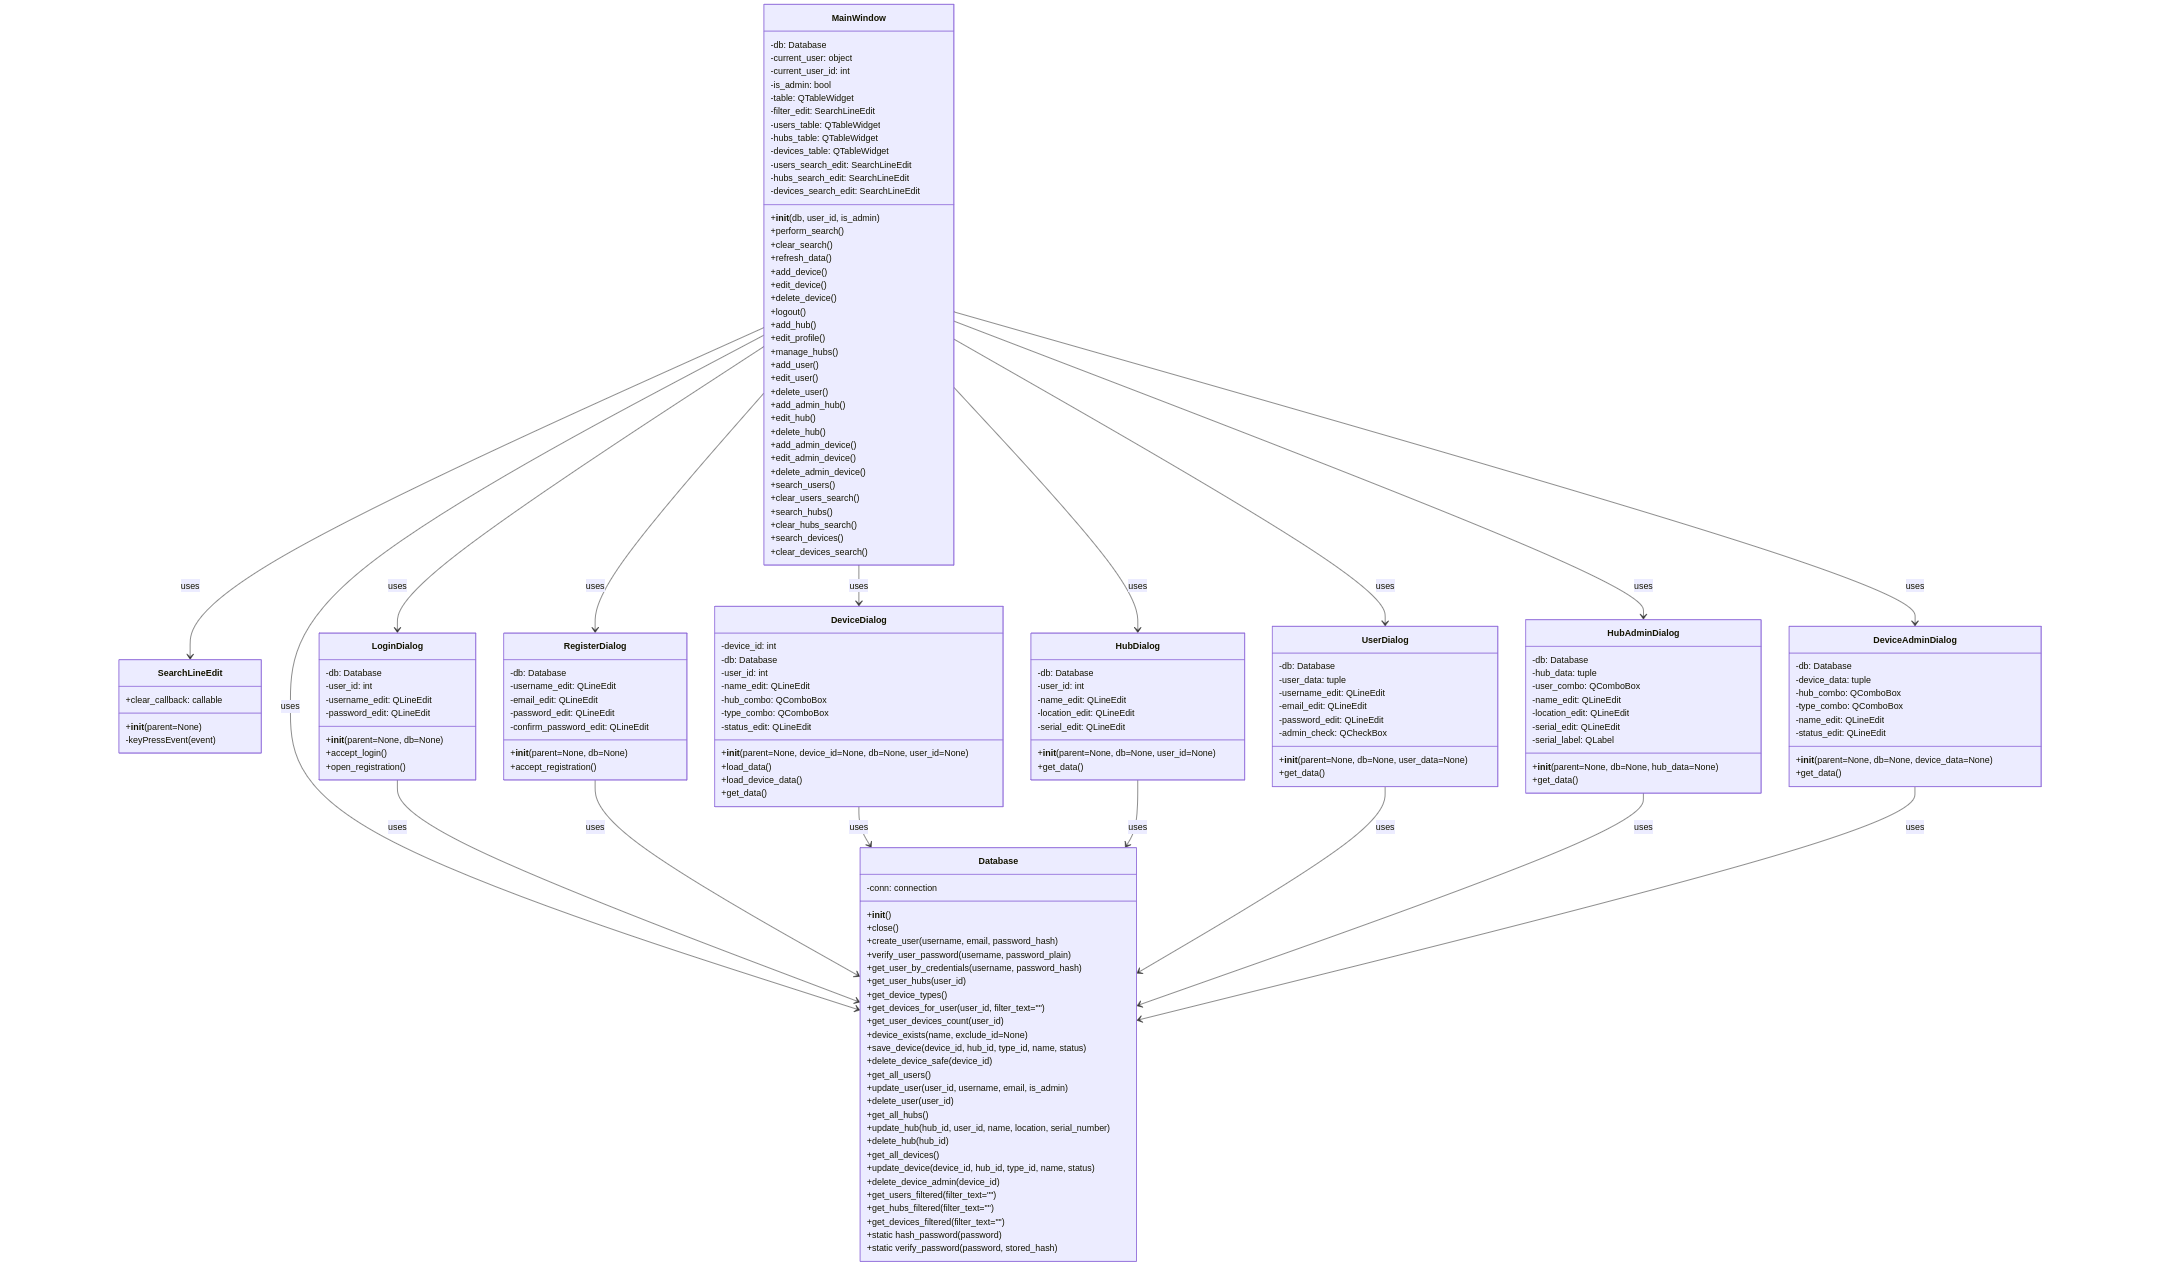
\includegraphics[width=0.9\textwidth]{pics/class_diagram.png}
  \caption{Диаграмма классов приложения}
\end{figure}

Диаграмма классов показывает архитектуру приложения и организацию работы с базой данных:
\begin{itemize}
  \item \texttt{Database} $-$ класс для подключения и выполнения операций с PostgreSQL
  \item \texttt{MainWindow} $-$ главное окно приложения с пользовательским интерфейсом
  \item \texttt{LoginDialog} $-$ диалог аутентификации пользователей
  \item \texttt{RegisterDialog} $-$ диалог регистрации новых пользователей
  \item \texttt{DeviceDialog} $-$ диалог управления устройствами
  \item \texttt{SearchLineEdit} $-$ кастомное поле поиска с поддержкой Esc
\end{itemize}

\subsection*{Подключение к базе данных}

\subsubsection*{Класс Database}
Центральный класс для работы с PostgreSQL, реализующий паттерн Singleton для управления соединением:

\begin{minted}{python}
import psycopg2
from psycopg2 import sql
import hashlib
import os

class Database:
    def __init__(self):
        # Установка соединения с PostgreSQL
        self.conn = psycopg2.connect(
            host="localhost",
            port=5433,
            database="pozordom",
            user="pozordom_user",
            password="pozordom_pass"
        )
        self.conn.autocommit = True
\end{minted}

\subsubsection*{Обработка исключений}
Реализована обработка всех типов ошибок подключения:

\begin{minted}{python}
def connect_to_database(self):
    try:
        self.db = Database()
        self.statusBar().showMessage("Подключено к базе данных")
    except Exception as e:
        QMessageBox.critical(self, "Ошибка подключения",
                           f"Не удалось подключиться к базе данных: {str(e)}")
\end{minted}

\subsection*{Выполнение запросов к БД}

\subsubsection*{Чтение данных}
Получение данных из таблиц с использованием параметризованных запросов:

\begin{minted}{python}
def get_devices_for_user(self, user_id, filter_text=""):
    query = """
        SELECT d.id, d.name, dt.type_name, h.name AS hub_name
        FROM devices d
        JOIN device_types dt ON d.type_id = dt.id
        JOIN hubs h ON d.hub_id = h.id
        WHERE h.user_id = %s AND d.name ILIKE %s
        ORDER BY d.id
    """
    with self.conn.cursor() as cur:
        cur.execute(query, (user_id, f"%{filter_text}%"))
        return cur.fetchall()
\end{minted}

\subsubsection*{Вставка и обновление данных}
Использование функции PL/pgSQL для безопасного сохранения:

\begin{minted}{python}
def save_device(self, device_id, hub_id, type_id, name, status):
    with self.conn.cursor() as cur:
        cur.callproc('save_devices', [device_id, hub_id, type_id, name, status])
        return cur.fetchone()[0]
\end{minted}

\subsubsection*{Удаление данных}
Безопасное удаление с очисткой связанных записей:

\begin{minted}{python}
def delete_device_safe(self, device_id):
    with self.conn.cursor() as cur:
        cur.execute("DELETE FROM log_devices WHERE device_id = %s", (device_id,))
        cur.execute("DELETE FROM devices WHERE id = %s", (device_id,))
\end{minted}

\subsection*{Работа с внешними ключами}

\subsubsection*{Загрузка связанных данных}
При добавлении устройств внешние ключи выбираются из списков:

\begin{minted}{python}
def load_data(self):
    hubs = self.db.get_user_hubs(self.user_id)
    self.hub_combo.clear()
    for hub_id, hub_name in hubs:
        self.hub_combo.addItem(hub_name, hub_id)

    device_types = self.db.get_device_types()
    self.type_combo.clear()
    for type_id, type_name in device_types:
        self.type_combo.addItem(type_name, type_id)
\end{minted}

\subsubsection*{Валидация уникальности}
Проверка отсутствия дубликатов перед сохранением:

\begin{minted}{python}
def device_exists(self, name, exclude_id=None):
    query = "SELECT 1 FROM devices WHERE name = %s"
    params = [name]
    if exclude_id:
        query += " AND id != %s"
        params.append(exclude_id)
    with self.conn.cursor() as cur:
        cur.execute(query, params)
        return cur.fetchone() is not None
\end{minted}

\subsection*{Ручной поиск с фильтрацией}

\subsubsection*{Регистронезависимый поиск}
Использование ILIKE для регистронезависимого поиска:

\begin{minted}{python}
def perform_search(self):
    filter_text = self.filter_edit.text().strip()
    devices = self.db.get_devices_for_user(self.current_user_id, filter_text)

    if not devices and filter_text:
        QMessageBox.warning(self, "Поиск",
                           f"Устройства с названием '{filter_text}' не найдены")
        return
\end{minted}

\subsubsection*{Подтверждение удаления}
Диалог подтверждения перед удалением устройств:

\begin{minted}{python}
reply = QMessageBox.question(
    self, "Подтверждение удаления",
    f"Вы действительно хотите удалить устройство '{device_name}'?",
    QMessageBox.StandardButton.Yes | QMessageBox.StandardButton.No,
    QMessageBox.StandardButton.No
)
\end{minted}

\subsection*{Скриншоты интерфейса}

\begin{figure}[H]
  \centering
  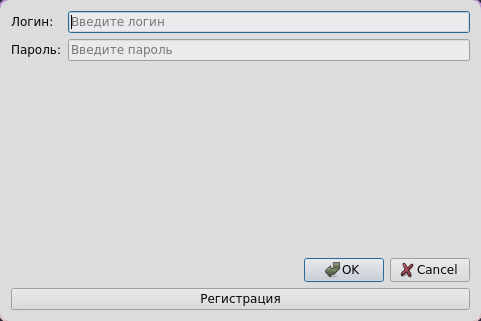
\includegraphics[width=0.8\textwidth]{pics/login.png}
  \caption{Рисунок 1 - Окно входа в систему}
\end{figure}

\begin{figure}[H]
  \centering
  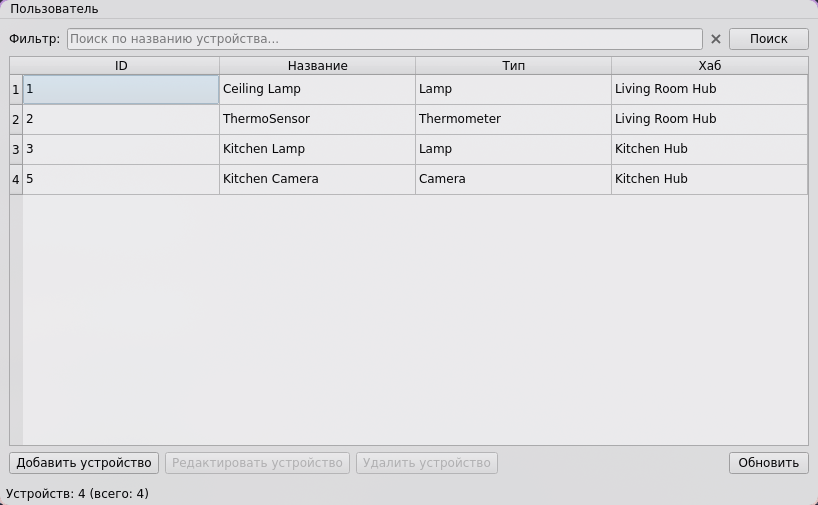
\includegraphics[width=0.8\textwidth]{pics/main_window.png}
  \caption{Рисунок 2 - Главное окно приложения}
\end{figure}

\begin{figure}[H]
  \centering
  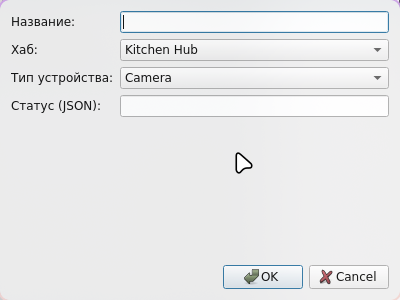
\includegraphics[width=0.8\textwidth]{pics/device_dialog.png}
  \caption{Рисунок 3 - Диалог добавления устройства}
\end{figure}

\begin{figure}[H]
  \centering
  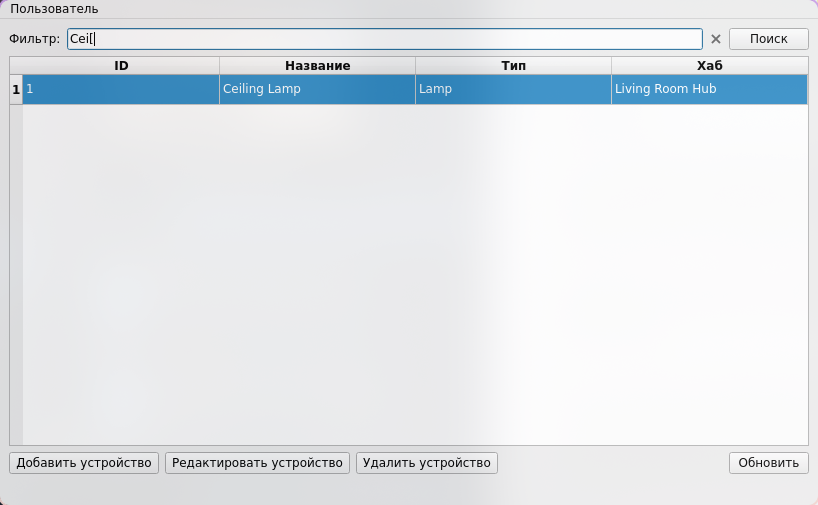
\includegraphics[width=0.8\textwidth]{pics/search_functionality.png}
  \caption{Рисунок 4 - Функционал ручного поиска}
\end{figure}

\section*{Вывод}

В ходе выполнения лабораторной работы №5 было освоено связывание приложения на Python с базой данных под управлением PostgreSQL. Разработано приложение с графическим интерфейсом, полностью соответствующее требованиям методических указаний:

\subsection*{Выполненные требования}

\subsubsection*{Требования к интерфейсу}
\begin{itemize}
  \item[$\checkmark$] Все названия колонок, кнопок и объектов интерфейса на русском языке
  \item[$\checkmark$] Реализован запрет ввода отрицательных значений (валидация ID и других числовых полей)
  \item[$\checkmark$] Регистронезависимый поиск с использованием ILIKE в SQL запросах
\end{itemize}

\subsubsection*{Работа с таблицей devices (содержит внешние ключи)}
\begin{itemize}
  \item[$\checkmark$] Вывод данных таблицы в табличном виде
  \item[$\checkmark$] Удаление записей с подтверждением пользователя
  \item[$\checkmark$] Изменение данных через диалоговое окно
  \item[$\checkmark$] Проверка дубликатов имен устройств перед сохранением
  \item[$\checkmark$] Фильтрация по названию устройства через SQL запросы
\end{itemize}

\subsubsection*{Работа с внешними ключами}
\begin{itemize}
  \item[$\checkmark$] При добавлении устройств hub\_id выбирается из списка хабов пользователя
  \item[$\checkmark$] type\_id выбирается из списка доступных типов устройств
  \item[$\checkmark$] Сохранение устройств через функцию PL/pgSQL save\_devices
  \item[$\checkmark$] Безопасное удаление с очисткой связанных записей в log\_devices
\end{itemize}

\subsubsection*{Техническая реализация}
\begin{itemize}
  \item[$\checkmark$] Фильтрация производится на уровне SQL запросов, а не в Python коде
  \item[$\checkmark$] Использование фреймворка PyQt6 для графического интерфейса
  \item[$\checkmark$] Применение паттернов проектирования для работы с БД
  \item[$\checkmark$] Обработка исключений и ошибок подключения
\end{itemize}

\subsection*{Ключевые особенности реализации}

\begin{enumerate}
  \item \textbf{Архитектура приложения}: Разделение на классы Database (работа с БД) и интерфейсные классы (PyQt6)
  \item \textbf{Безопасность данных}: Параметризованные запросы, предотвращение SQL инъекций
  \item \textbf{Удобство использования}: Ручной поиск с кнопкой "×" и поддержкой Esc для очистки
  \item \textbf{Целостность данных}: Использование транзакций и функций PL/pgSQL
  \item \textbf{Масштабируемость}: Модульная архитектура, легко расширяемая для новых функций
\end{enumerate}

Приложение полностью соответствует требованиям лабораторной работы №5 и демонстрирует правильное связывание Python приложения с PostgreSQL базой данных.

\newpage

\section*{Приложение А1. Исходный код main.py}
\inputminted{python}{code/main.py}

\section*{Приложение А2. Исходный код database.py}
\inputminted{python}{code/database.py}

\section*{Приложение А3. Файл зависимостей}
\inputminted{text}{code/requirements.txt}

\end{document}
